\documentclass[12pt]{article}

%%%%%%%%%%%%%%%%%%%%%%%%%%%%%%%%%%%%%%%%%%%%%%%%%%%
%%%%%%%%%%%%%%%%%Packages%%%%%%%%%%%%%%%%%%%%%%%%%%
%%%%%%%%%%%%%%%%%%%%%%%%%%%%%%%%%%%%%%%%%%%%%%%%%%%

\usepackage[T1]{fontenc}
\usepackage{tikz, tkz-euclide}
\usepackage{pgfplots}
\usepgfplotslibrary{groupplots}
\usetikzlibrary{shapes,arrows}
\usepackage{mathpazo}
\usepackage{graphicx}
\usepackage{caption}
\usepackage{adjustbox}
\usepackage{xcolor}
\usepackage{enumerate}
\usepackage{geometry}
\usepackage{amsmath} 
\usepackage{amssymb} 
\usepackage{textcomp}
\usepackage{upquote}
\usepackage[mathletters]{ucs}
\usepackage[utf8x]{inputenc}
\usepackage[english]{babel}
\usepackage[T1]{fontenc}
\usepackage{amsmath,amssymb,bm}
\usepackage{hyperref}
\usepackage{color}
\usepackage{listings}
\usepackage{subfig}
\usepackage{placeins}
\usepackage{systeme}
\usepackage{amsthm}
\usepackage{float}

\lstset{
	backgroundcolor=\color[rgb]{0.86,0.88,0.93},
	language=Python, keywordstyle=\color[rgb]{0,0,1},
	basicstyle=\footnotesize \ttfamily,breaklines=true,
	escapeinside={\%*}{*)},
	numbers=left
}

%%%%%%%%%%%%%%%%%%%%%%%%%%%%%%%%%%%%%%%%%%%%%%%
%%%%%%%%%%%%%%Theorem Environments%%%%%%%%%%%%%
%%%%%%%%%%%%%%%%%%%%%%%%%%%%%%%%%%%%%%%%%%%%%%%

\newcounter{LemmaCounter}
\newcounter{TheoremCounter}
\newcounter{CorollaryCounter}
\newcounter{DefinitionCounter}
\newcounter{PropositionCounter}

\newtheorem{Definition}[DefinitionCounter]{Definition}
\newtheorem{Lemma}[LemmaCounter]{Lemma}
\newtheorem{Theorem}[TheoremCounter]{Theorem}
\newtheorem{Corollary}[CorollaryCounter]{Corollary}
\newtheorem{Proposition}[PropositionCounter]{Proposition}

%%%%%%%%%%%%%%%%%%%%%%%%%%%%%%%%%%%%%%%%%%%%%%%%%%%
%%%%%%%%%%%%%%%%%%Document%%%%%%%%%%%%%%%%%%%%%%%%%
%%%%%%%%%%%%%%%%%%%%%%%%%%%%%%%%%%%%%%%%%%%%%%%%%%%

\begin{document}
	\title{Lecture Notes on Control Theory: Time response}
	
	\vskip0.8cm
	
	\author{Eduardo Fernandes 
		Montesuma \\ email \href{mailto:edumontesuma@gmail.com}{edumontesuma@gmail.com}}
	
	\date{19/04/2018}
	
	\maketitle
	
	\tableofcontents
	
	\newpage
	
	\section{Exercise 1}
		Consider the following mechanical system,
		
		\begin{figure}[H]
			\centering
			\includegraphics[scale=0.5]{img1}
			\caption{System schematic for exercise 1}
			\label{Figure 1}
		\end{figure}
	
		To use Newton's second law, we point out that, by Hooke's law the force done by the spring is $F_{e} = -kx(t)$, also, the force done by the damp is $F_{d} = -b\dot{x}(t)$. Therefore, by Newton's Second law,
		
		\begin{align*}
			\sum F &= m\ddot{x}\\
			f -b\dot{x} - kx &= m\ddot{x}\\
			f &= m\ddot{x} + b\dot{x} + kx
		\end{align*}
		
		Which is the ODE that describes our system. To find its transfer function, suppose that $x(0) = 0$ and $\dot{x}(0) = 0$. So,
		
		\begin{align*}
			ms^{2}X(s) + bsX(s) + kX(s) &= F(s)\\
			(ms^{2} + bs + k)X(s) &= F(s)\\
			\dfrac{X(s)}{F(s)} &= \dfrac{1}{ms^{2} + bs + k}
		\end{align*}
		
		Now, to analyze it in the time domain, we need to find parameters $\zeta$ and $\omega_{n}$ such that,
		
		\begin{align*}
			\dfrac{1}{ms^{2} + bs + k} &= \dfrac{\omega_{n}^{2}}{s^{2} + 2\zeta \omega_{n}s + \omega_{n}^{2}}
		\end{align*}
		
		To do so, we manipulate the expression for our transfer function,
		
		\begin{align*}
			\dfrac{1}{ms^{2} + bs + k} &= \dfrac{1/m}{s^{2} + (b/m)s + k/m}
		\end{align*}
		
		Then, $\omega_{n} = \biggr(\dfrac{k}{m}\biggr)^{1/2}$, therefore, $2\zeta\omega_{n} = \dfrac{b}{m}$, that is,
		
		\begin{align*}
			\zeta &= \dfrac{b}{2m\omega_{n}}\\
			\zeta &= \dfrac{b}{2m}\dfrac{m^{1/2}}{k^{1/2}}\\
			\zeta &= \dfrac{b}{2\sqrt{mk}}
		\end{align*}
		
		In terms of values, those are: $\zeta = 0.211$ and $\omega_{n} = 2.366$. Now we need to calculate four quantities,
		
		\begin{itemize}
			\item The settling time, given by the time needed for $x(t)$ to be on a interval of $1\%$ of its steady state value,
			\item The overshoot in percentage, given by the percentage that the response exceed its steady state value and,
			\item The peak time, given by the time at which the response achieve its maximum value.
		\end{itemize}
	
		The settling time can be calculated using the formula $t_{s} = \dfrac{4}{\zeta \omega_{n}} = 8s$. The overshoot is calculated by $\%OS = exp\biggr(\dfrac{-\pi\zeta}{\sqrt{1-\zeta^{2}}}\biggr)\times 100 = 50.70\%$. Finally, the peak time is given by $t_{p} = \dfrac{4.6}{\zeta \omega_{n}} = 9.2s$
	\section{Exercise 3}
		For such exercise, we have two transfer functions,
		
		\begin{align}
			C_{1}(s) &= \dfrac{26.25(s+4)}{s(s+3.5)(s+5)(s+6)}\\
			C_{2}(s) &= \dfrac{26.25(s+4)}{s(s+4.01)(s+5)(s+6)}
		\end{align}
		
		none of these transfer functions have pole-zero cancellations, but they can be approximated as there were. Particularly, we make the approximation
		
		\begin{align*}
			\tilde{C} = \dfrac{26.25}{s(s+5)(s+6)}
		\end{align*}
		
		and plot the results to analyze if our approximation is close to the real systems. We can see this graphically, bellow,
		
		\begin{figure}[H]
			\centering
			\includegraphics[width = \textwidth]{img2}
			\caption{On the left, $C_{1}$ and $\tilde{C}$. On the right, $C_{2}$ and $\tilde{C}$.}
			\label{Figure 2}
		\end{figure}
	
		these plots provide us graphical information about our approximation: $\tilde{C}$ approximates much better $C_{2}$ than $C_{1}$, as we expected. To give some numerical insight, we calculate the Root Mean Squared Error (RMSE) between $C_{1}$ and $\tilde{C}$, as well as between $C_{2}$ and $\tilde{C}$. The RMSE is defined as,
		
		\begin{align*}
			RMSE(C_{i},\tilde{C}) &= \dfrac{1}{n}\sqrt{\sum_{j=1}^{n}(C_{ij}-\tilde{C}_{j})}
		\end{align*}
		
		thus, it gives us a numeric insight of how much $C_{i}$ deviates from $\tilde{C}$. Effectively, $RMSE(C_{1},\tilde{C}) = 1.25\times 10^{-4}$ and $RMSE(C_{2},\tilde{C}) = 1.52\times 10^{-6}$, in accordance with our graphical results.
	\section{Exercise 4}
		Consider the following state space representation of a system,
		
		\begin{align*}
			\begin{cases}
				\dot{\mathbf{x}}(t) &= \begin{bmatrix}
				0 & 2\\
				-3 & -5
				\end{bmatrix}\mathbf{x}(t) + \begin{bmatrix}
				0\\
				1
				\end{bmatrix}e^{-t}\\
				y(t) &= \begin{bmatrix}
					1 & 3
				\end{bmatrix}\mathbf{x}(t)
			\end{cases}\\
			\mathbf{x}(0) = \begin{bmatrix}
				1\\
				0
			\end{bmatrix}
		\end{align*}
			
		to get, from such representation, the laplace transform, we need to calculate the expression,
		
		\begin{align*}
			T(s) &= \mathbf{C}(s\mathbf{I} - \mathbf{A})^{-1}\mathbf{B} + \mathbf{D}
		\end{align*}
		
		where,
		
		\begin{align*}
			(s\mathbf{I}-\mathbf{A})^{-1} &= \begin{bmatrix}
				\dfrac{s+5}{s^{2}+5s+6} & \dfrac{2}{s^{2}+5s+6}\\
				\dfrac{-3}{s^{2}+5s+6} & \dfrac{s}{s^{2}+5s+6}
			\end{bmatrix}\\
			\mathbf{B} &= \begin{bmatrix}
				0\\
				1
			\end{bmatrix}\\
			\mathbf{C} &= \begin{bmatrix}
				1 & 3
			\end{bmatrix}\\
			\mathbf{D} &= \mathbf{0}
		\end{align*}
		
		Being so,
		
		\begin{align*}
			T(s) &= \begin{bmatrix}
				1 & 3
			\end{bmatrix}\begin{bmatrix}
			\dfrac{s+5}{s^{2}+5s+6} & \dfrac{2}{s^{2}+5s+6}\\
			\dfrac{-3}{s^{2}+5s+6} & \dfrac{s}{s^{2}+5s+6}
			\end{bmatrix}\begin{bmatrix}
				0\\
				1
			\end{bmatrix}\\
			&= \begin{bmatrix}
			1 & 3
			\end{bmatrix}\begin{bmatrix}
				\dfrac{2}{s^{2}+5s+6}\\
				\dfrac{s}{s^{2}+5s+6}
			\end{bmatrix} = \dfrac{3s + 2}{s^{2}+5s+6}
		\end{align*}
		
		now, we need to solve this system in the light of a complete response with $u(t) = e^{-t}$. To do so, we need to evaluate the free-response, and the forced response. Computing the first, we notice that the I/O model of our system is,
		
		\begin{align*}
			Y(s) &= T(s)U(s)\\
			(s^{2}+5s+6)Y(s) &= (3s+2)U(s)\\
			\ddot{y} + 5\dot{y} + 6y &= 3\dot{u} + 2u
		\end{align*}
		
		concerning the initial conditions, we can calculate $y(0)$ by using the output equation in the State-Space model for $t = 0$,
		
		\begin{align*}
			y(0) &= \begin{bmatrix}
				1 & 3
			\end{bmatrix}\mathbf{x}(0)\\
				 &= \begin{bmatrix}
				 1 & 3
				 \end{bmatrix}\begin{bmatrix}
					 1\\
					 0
				 \end{bmatrix} = 1
		\end{align*}
		
		finally, we calculate the free-response using the Laplace transform,
		
		\begin{align*}
			s^{2}Y(s) - s + 5sY(s) - 5 + 6Y(s) = 0\\
			Y(s) = \dfrac{s+5}{s^{2}+5s+6} = \dfrac{s+5}{(s+3)(s+2)}
		\end{align*}
		
		by fraction expansions, we have,
		
		\begin{align*}
			A &= \lim\limits_{s \rightarrow -3}\dfrac{s+5}{s+2} = -2\\
			B &= \lim\limits_{s \rightarrow -2}\dfrac{s+5}{s+3} = 3
		\end{align*}
		
		that is,
		
		\begin{align*}
			Y(s) &= \dfrac{-2}{s+3} + \dfrac{3}{s+2}\\
			y_{free}(t) &= 3e^{-2t} - 2e^{-3t}
		\end{align*}
		
		Now, for the forced response, we have $U(s) = \dfrac{1}{s+1}$. Using our transfer function,
		
		\begin{align*}
			Y(s) &= T(s)U(s)\\
				 &= \dfrac{3s+2}{(s+1)(s+2)(s+3)}
		\end{align*}
		
		working with fraction expansions again,
		
		\begin{align*}
			A &= \lim\limits_{s\rightarrow -1}\dfrac{3s+2}{(s+2)(s+3)} = \dfrac{-1}{2}\\
			B &= \lim\limits_{s\rightarrow -2}\dfrac{3s+2}{(s+1)(s+3)} = 4\\
			A &= \lim\limits_{s\rightarrow -3}\dfrac{3s+2}{(s+1)(s+2)} = \dfrac{-7}{2}
		\end{align*}
		
		that is,
		
		\begin{align*}
			y_{forced}(t) &= \dfrac{1}{2}\biggr(-2e^{-t}+8e^{-2t} -7e^{-3t}\biggr)
		\end{align*}
		
		the complete response, finally, is the sum of those latter two,
		
		\begin{align*}
			y_{complete}(t) &= y_{free}(t) + y_{forced}(t)\\
							&= \dfrac{1}{2}\biggr(14e^{-2t}  - 11e^{-3t} - 2e^{-t}\biggr)
		\end{align*}
		
		\begin{figure}[H]
			\centering
			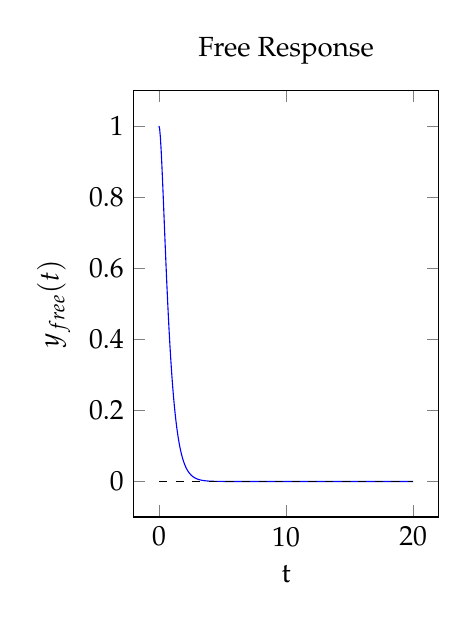
\begin{tikzpicture}
			\begin{axis}[title = {Free Response}, ylabel = {$y_{free}(t)$}, xlabel = {t}
			,width = 0.45*\textwidth, height = 7cm]
			\addplot [domain = 0:20, samples = 350, blue]{3*exp(-2*\x)-2*exp(-3*\x)};
			\addplot [domain = 0:20, dashed]{0};
			\end{axis}
			\end{tikzpicture}
			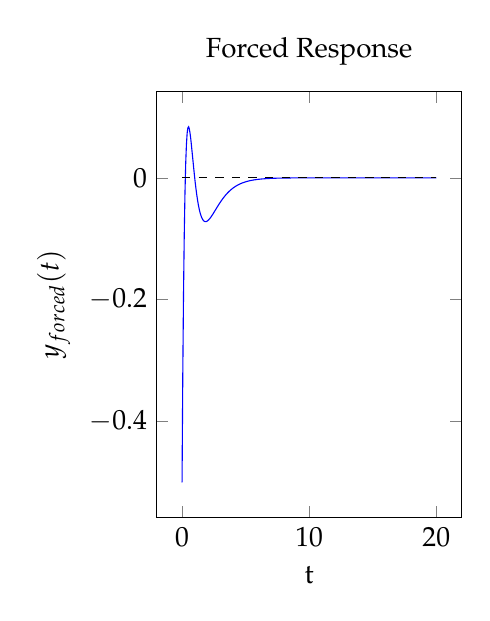
\begin{tikzpicture}
			\begin{axis}[title = {Forced Response}, ylabel = {$y_{forced}(t)$}, xlabel = {t}, width = 0.45*\textwidth, height = 7cm]
				\addplot [domain = 0:20, samples = 350, blue]{0.5*(-2*exp(-\x)+8*exp(-2*\x)-7*exp(-3*\x))};
				\addplot [domain = 0:20, dashed]{0};
			\end{axis}
			\end{tikzpicture}
			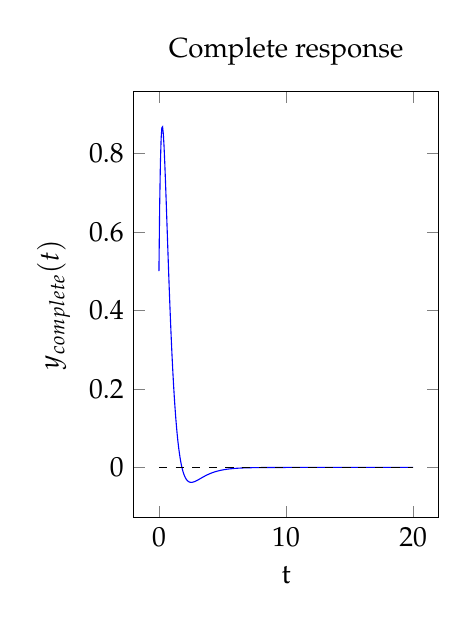
\begin{tikzpicture}
			\begin{axis}[title = {Complete response}, ylabel = {$y_{complete}(t)$}, xlabel = {t},width = 0.45*\textwidth, height = 7cm]
			\addplot [domain = 0:20, samples = 350, blue]{0.5*(-2*exp(-\x)+14*exp(-2*\x)-11*exp(-3*\x))};
			\addplot [domain = 0:20, dashed]{0};
			\end{axis}
			\end{tikzpicture}
			\caption{The plot of each response}
			\label{Figure 3}
		\end{figure}
		
		Finally, the poles of our system are $-2$ and $-3$, which coincide with the eigenvalues of $\mathbf{A}$. This comes from the fact that, in the algorithm for matrix inversion, we need to calculate the determinant of $(s\mathbf{I}-A)$, which goes on the denominator of the transfer function. From elementary linear algebra, we know that the solutions of $det(s\mathbf{I}-A) = 0$ are the eigenvalues of $\mathbf{A}$.
		
		Now, we need to calculate $\Phi(t) = e^{\mathbf{A}t}$, which is given by,
		
		\begin{align*}
			\Phi(t) &= \begin{bmatrix}
				K_{1}e^{-2t} + K_{2}e^{-3t} & K_{3}e^{-2t} + K_{4}e^{-3t}\\
				K_{5}e^{-2t} + K_{6}e^{-3t} & K_{7}e^{-2t} + K_{8}e^{-3t}\\
			\end{bmatrix}
		\end{align*}
		
		With coefficients $K_{1},\cdots,K_{8}$ to determine. Also, notice that $\Phi(0) = \mathbf{I}$, and $\dfrac{d}{dt}\Phi(t)\biggr\vert_{t = 0} = \mathbf{A}e^{\mathbf{A}t}\biggr\vert_{t = 0} = \mathbf{A}$. Using those equations,
		
		\begin{align*}
			&K_{1} + K_{2} = 1& &K_{3}+K_{4} = 0&\\
			&-2K_{1}-3K_{2} = 0& &-2K_{3}-3K_{4}= 2&\\
			&K_{5} + K_{6} = 0& &K_{7}+K_{8} = 1&\\
			&-2K_{5} - 3K_{6} = -3& &-2K_{7}-3K_{8} = -5&
		\end{align*}
		
		which yields,
		
		\begin{align*}
			&K_{1} = 3& &K_{2} = -2& &K_{3} = 2& &K_{4} = -2& \\
			&K_{5} = -3& &K_{6} = 3& &K_{7} = 8& &K_{8} = -7&
		\end{align*}
		
		That is,
		
		\begin{align*}
			\Phi(t) &= \begin{bmatrix}
				3e^{-2t}-2e^{-3t} & 2e^{-2t} - 2e^{-3t}\\
				-3e^{-2t}+3e^{-3t} & 8e^{-2t} - 7e^{-3t}
			\end{bmatrix}
		\end{align*}
		
		Still, this is only one way to calculate $\Phi(t)$. Other way is to apply the inverse Laplace transform to each element of $(s\mathbf{I}-\mathbf{A})^{-1}$, which is a good exercise. Up to now, you should be convinced by these examples that these two ways of represent systems are equivalent.
		
	\section{Exercise 5}
		As discussed before, to find the eigenvalues of $\mathbf{A}$ is equivalent to find the poles of the transfer function associated with the State-Space representation. Being so, we work only with the eigenvalues.
		
		First, notice that we need to calculate the determinant $det(s\mathbf{I}-A)$, that is,
		
		\begin{align*}
			\begin{vmatrix}
				s & -1 & 0\\
				0 & s & -1\\
				24 & 26 & s+9
			\end{vmatrix} &= s^{2}(s+9) + 24 - 24s + 26s\\
						&= s^{3} + 9s^{2} + 2s + 24
		\end{align*}
		
		which has as roots $s_{1} = -9.0712$, $s_{2} = 0.0356 - 1.6262i$ and $s_{3} = 0.0356 + 1.6262i$\footnote{Roots were computed numerically}.
	\section{Extra: solving state space equations}
		\subsection{Introduction}
		We want to develop a theory to treat a general, closed form solution for any  first order (scalar) ordinary differential equation (ODE) because, as we shall see later on, an n-order ODE can be written as a first-order (vectorial) ODE. We start with the simplest kind of ODE, namely:
		
		\begin{align}
		\dfrac{dx(t)}{dt} &= Ax(t) \label{Equation 1}
		\end{align}
		
		Here, the solution is straight-forward using the fundamental theorem of calculus, after noticing $\dfrac{d}{dt}[log(x(t))] = \dfrac{1}{x}\dfrac{dx}{dt}$:
		
		\begin{align}
		\dfrac{1}{x}\dfrac{dx}{dt} &= A\\
		\dfrac{d}{dt}log[x(t)] &= A\\
		log[x(t)] &= At + C_{1}\\
		x(t) &= e^{At + C_{1}}\\
		x(t) &= C_{2}e^{At}
		\end{align}
		
		Where we have used the notation $C_{2} = e^{C_{1}}$. The solution, to be precisely is a family of solutions, indexed by two parameters, $C_{2}$ and $A$:
		
		\begin{align}
		x(t|A,C) &= Ce^{At}
		\end{align}			
		
		\begin{figure}[H]
			\centering
			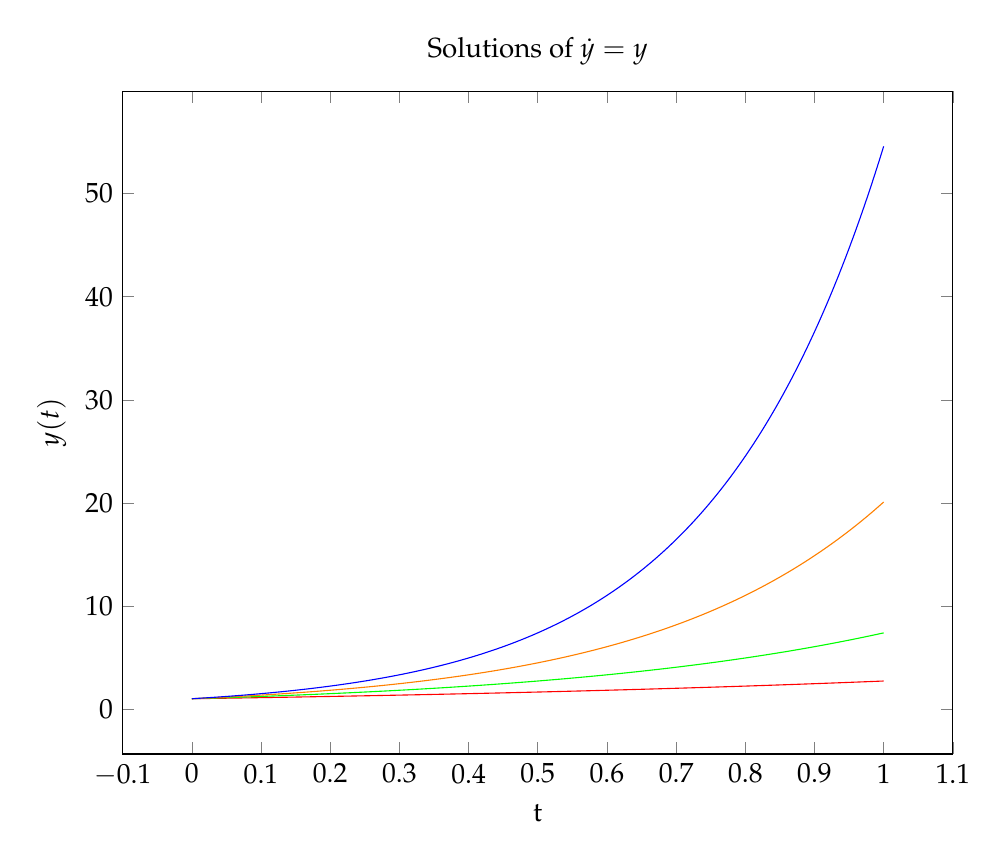
\begin{tikzpicture}
			\begin{axis}[title = {Solutions of $\dot{y}=y$}, ylabel = {$y(t)$}, xlabel = {t}
			,width = \textwidth, height = 10cm]
			\addplot [domain = 0:1, samples = 200, red]{exp(\x)};
			\addplot [domain = 0:1, samples = 200, green]{exp(2*\x)};
			\addplot [domain = 0:1, samples = 200, orange]{exp(3*\x)};
			\addplot [domain = 0:1, samples = 200, blue]{exp(4*\x)};
			\end{axis}
			\end{tikzpicture}
			\caption{Form of solution's family}
			\label{Figure 4}
		\end{figure}
		
		The shape of solutions, for each choice of parameters $(A,C)$ is given in Figure \ref{Figure 4}. Although simple, the methodology to solve this particular kind of ODE can be carried out for more complex cases, that is, we try to manipulate the ODE in order to achieve some integrable function. This is exactly the nature of the integrating factor method, which is now discussed.
		
		\subsection{First-Order linear ODEs}
		The last case was a simple sub-case of a much more wider class of differential equations: the linear ones. A linear first-order ODE is given by,
		
		\begin{align}
		\dot{x}(t) + p(t)x(t) &= q(t)
		\end{align}
		
		where $p(t)$ and $q(t)$ are sufficiently smooth functions\footnote{We mean by "sufficiently smooth" functions that are both continuous and differentiable.}. Again, recalling the last paragraph of last section, we want to express the left hand side as a derivative of something. 
		
		By force, we want to multiply the ODE by a function $\mu(t)$ such that $\mu(t)(\dot{x}(t)+p(t)x(t)) = \dfrac{d}{dt}\biggr(\mu(t)x(t)\biggr)$, that is,
		
		\begin{align}
		\dot{\mu}x + \mu\dot{x} &= \mu\dot{x} + \mu(t)p(t)x(t)\\
		\dot{\mu}x(t) &= \mu(t)p(t)x(t)\\
		\dfrac{\dot{\mu}}{\mu} &= p\\
		\int_{t_{0}}^{t} \dfrac{\dot{\mu}(t)}{\mu} &= \int_{t_{0}}^{t} p(\tau)d\tau\\
		log\text{ }\mu(t) &= \int_{t_{0}}^{t} p(\tau)d\tau\\
		\mu(t) &= e^{\int_{t_{0}}^{t} p(\tau)d\tau}
		\end{align}
		
		Putting it back into the ODE,
		
		\begin{align}
		\dfrac{d}{dt}\biggr(x(t)e^{\int_{t_{0}}^{t}p(\tau)d\tau} \biggr) &= q(t)e^{\int_{t_{0}^{t}}p(\tau)d\tau }\\
		x(t)e^{\int_{t_{0}}^{t}p(\tau)d\tau} - x(t_{0})e^{\int_{t_{0}}^{t_{0}}p(\tau)d\tau} &= \int_{t_{0}}^{t}q(r)e^{\int_{t_{0}}^{r}p(\tau)d\tau}dr
		\end{align}
		
		And therefore, the solution takes form:
		
		\begin{align}
		x(t) &= x(t_{0})e^{-\int_{t_{0}}^{t}p(\tau)d\tau} + e^{-\int_{t_{0}}^{t}p(\tau)d\tau}\int_{t_{0}}^{t}q(r)e^{\int_{t_{0}}^{r}p(\tau)d\tau}dr
		\end{align}
		
		Such a solution is valid for any functions $p(t)$ and $q(t)$ satisfying our constraints. In practice, to describe systems with those concepts is to consider between the following classifications,
		
		\begin{itemize}
			\item Time-Invariant systems, in which $p(t) = a$, $q(t) = b$, for all $t \in \mathbb{R}$.
			\item Homogeneous systems, in which $q(t) = 0$.
		\end{itemize}
		
		For each of those classifications, there comes assumptions which simplifies our equations.
	
	\subsection{Linear and Homogeneous case}
	Consider a differential equation of $n^{th}$ order. For now, let us consider the linear homogeneous case, that is,
	
	\begin{align}
	\dfrac{d^{n}x}{dt^{n}} + a_{n-1}\dfrac{d^{n-1}x}{dt^{n-1}} + \cdots + a_{1}\dfrac{dx}{dt} + a_{0} &= 0
	\end{align}
	
	We can transform this equation into a system of equations, using the following notation,
	
	\begin{align}
	x_{1} &= x & \dot{x}_{1} &= \dfrac{dx}{dt}\\
	x_{2} &= \dfrac{dx}{dt} & \dot{x}_{2} &= \dfrac{d^{2}x}{dt^{2}}\\
	\vdots\\
	x_{n} &= \dfrac{d^{n-1}x}{dt^{n-1}} & \dot{x}_{n} &= \dfrac{d^{n}x}{dt^{n}}
	\end{align}
	
	Noticing that $\dot{x}_{j} = x_{j+1}$, for $0 \leq j < n$, and that $\dot{x}_{n} = \dfrac{d^{n}x}{d^{n}t} = \sum_{j}(-a_{j})x_{j}$, we can express the system through matrices:
	
	\begin{align}
	\begin{bmatrix}
	\dot{x}_{1}\\
	\dot{x}_{2}\\
	\vdots\\
	\dot{x}_{n}
	\end{bmatrix}
	&=
	\begin{bmatrix}
	0 & 1 & 0 & \cdots & 0\\
	0 & 0 & 1 & \cdots & 0\\
	\vdots & \vdots & \vdots & \cdots & \vdots\\
	-a_{0} & -a_{1} & -a_{2} & \cdots & -a_{n-1}
	\end{bmatrix}\begin{bmatrix}
	x_{1}\\
	x_{2}\\
	\vdots\\
	x_{n}
	\end{bmatrix}\\
	\dot{\mathbf{x}} &= \mathbf{Ax} \label{Equation 24}
	\end{align}
	
	Notice that this later differential equation resembles Equation \ref{Equation 1}. We argue that the solution of such a system is $\mathbf{x}(t) = \mathbf{x}(0)e^{\mathbf{A}t}$, just as before, but with the exponential of a matrix. 
	
	Before prove our claim, we shall provide the definition of matrix exponentials. Looking at the scalar case, through Taylor series, the exponential function can be expressed as:
	
	\begin{align}
	e^{at} &= 1 + \sum_{n=1}^{\infty}\dfrac{a^{n}t^{n}}{n!}
	\end{align}
	
	Under the assumption of convergence, this series gives us the given exponential. If we instead consider matrices, we can write:
	
	\begin{align}
	e^{\mathbf{A}t} &= \mathbf{I} + \sum_{n=1}^{\infty}\dfrac{\mathbf{A}^{n}t^{n}}{n!}
	\end{align}
	
	Where the convergence is done element-wise. Consider, now, the derivative:
	
	\begin{align}
	\dfrac{d}{dt}e^{\mathbf{A}t} &= \dfrac{d}{dt}\mathbf{I} + \sum_{n=1}^{\infty}\dfrac{\mathbf{A}^{n}}{n!}\dfrac{d}{dt}t^{n}\\
	&= \sum_{n=1}^{\infty}\dfrac{\mathbf{A}^{n}}{(n-1)!}t^{n-1}\\
	&= \mathbf{A}\biggr(\mathbf{I} + \sum_{n=1}^{\infty}\dfrac{\mathbf{A}^{n}t^{n}}{n!}\biggr)\\
	&= \mathbf{A}e^{\mathbf{A}t}
	\end{align} 
	
	Therefore, if $\mathbf{x}(t) = \mathbf{x}(0)e^{\mathbf{A}t}$, we can write:
	
	\begin{align}
	\dfrac{d}{dt}\mathbf{x}(t) &= \mathbf{x}(0)\dfrac{d}{dt}e^{\mathbf{A}t}\\
	&= \mathbf{A}(\mathbf{x}(0)e^{\mathbf{A}t})\\
	&= \mathbf{A}\mathbf{x}(t)
	\end{align}
	
	As we wanted. This case is indeed simple and without complications, since $A$ does not depend on time, and the equation is homogeneous. We shall explore more complex cases henceforth.
	\subsection{Non-homogeneous time-invariant}
	In that case, we are considering the following ODE:
	
	\begin{align}
	\dot{\mathbf{x}}(t) &= \mathbf{Ax}(t) + \mathbf{Bu}(t)
	\end{align}
	
	for a sufficiently smooth function $\mathbf{u}:\mathbb{R}\rightarrow\mathbb{R}^{n}$. To solve such a system, we perform just like we have done with the integrating factor\footnote{indeed, $\mu(t) = e^{-\int_{0}^{t}\mathbf{A}(\tau)d\tau}$, which leaves us with $e^{-\mathbf{A}t}$}:
	
	\begin{align}
	e^{-\mathbf{A}t}\dot{\mathbf{x}}(t) - e^{-\mathbf{A}t}\mathbf{A}\mathbf{x}(t)&= e^{-\mathbf{A}t}\mathbf{Bu}(t)
	\end{align}
	
	Noticing that $\dfrac{d}{dt} e^{\mathbf{A}t}\mathbf{x}(t)$ yields the right-hand-side (RHS) of such equation,
	
	\begin{align}
	\dfrac{d}{dt}e^{-\mathbf{A}t}\mathbf{x}(t) &= e^{-\mathbf{A}t}\mathbf{Bu}(t)\\
	e^{-\mathbf{A}t}\mathbf{x}(t) - e^{-\mathbf{A}t_{0}}\mathbf{x}_{0}(t_{0}) &= \int_{t_{0}}^{t}e^{-\mathbf{A}\tau}\mathbf{Bu}(\tau)d\tau 
	\end{align}
	
	Rearranging, gives us the full solution for the time-invariant system,
	
	\begin{align}
	\mathbf{x}(t) &= e^{\mathbf{A}(t-t_{0})}\mathbf{x}_{0}(t_{0}) + \int_{t_{0}}^{t}e^{\mathbf{A}(t-\tau)}\mathbf{Bu}(\tau)d\tau
	\end{align}
	
	As we shall see in the next section, this is the solution for the state equations of time-invariant systems.
	\subsection{Non-homogeneous time-variant}
	This is the most general case for linear systems. they are governed by the ODE,
	
	\begin{align}
	\dot{\mathbf{x}} &= \mathbf{A}(t)\mathbf{x}(t) + \mathbf{B}(t)\mathbf{u}(t)
	\end{align}
	
	For such equation, however, the solution is not straightforward as before, since we need to solve the integrating factor
	
	\begin{align}
	\mu(t) &= e^{-\int_{t_{0}}^{t}\mathbf{A}(\tau)d\tau}
	\end{align}
	
	Indeed, we shall rather represent $\mu(t)$ as a transition matrix, between time $t_{0}$ and $t$,
	
	\begin{align}
	\Phi(t,t_{0}) &= e^{-\int_{t_{0}}^{t}\mathbf{A}(\tau)d\tau}
	\end{align}
	
	Which has the following properties,
	
	\noindent\textbf{Property 1:} $\dfrac{\partial \Phi}{\partial t} = -\Phi(t,t_{0})\mathbf{A}(t)$
	
	\noindent\textit{Proof:} By our definition,
	
	\begin{align}
	\dfrac{\partial \Phi}{\partial t} &= \dfrac{\partial}{\partial t}e^{-\int_{t_{0}}^{t}\mathbf{A}(\tau)d\tau}\\
	&= e^{-\int_{t_{0}}^{t}\mathbf{A}(\tau)d\tau}\dfrac{d}{dt}\biggr(-\int_{t_{0}}^{t}\mathbf{A}(\tau)d\tau\biggr)\\
	&= -\Phi(t,t_{0})\mathbf{A}(t)
	\end{align}
	
	Where from the first equation, from the second, we have used the matrix exponential derivative with the chain rule.
	\\
	\\
	\noindent\textbf{Property 2:} $\dfrac{\partial \Phi}{\partial t_{0}} = \mathbf{A}(t)\Phi(t,t_{0})$
	\\
	\\
	\noindent\textit{Proof:} Again, using the definition,
	
	\begin{align}
	\dfrac{\partial \Phi}{\partial t} &= \dfrac{\partial}{\partial t_{0}}e^{-\int_{t_{0}}^{t}\mathbf{A}(\tau)d\tau}\\
	&= \dfrac{d}{dt_{0}}\biggr(-\int_{t_{0}}^{t}\mathbf{A}(\tau)d\tau\biggr)e^{-\int_{t_{0}}^{t}\mathbf{A}(\tau)d\tau}\\
	&= \mathbf{A}(t)\Phi(t,t_{0})
	\end{align}
	
	Now, proceeding as before, 
	
	\begin{align}
	e^{-\int_{0}^{t}\mathbf{A}(\tau)d\tau}\dot{\mathbf{x}}(t) - e^{-\int_{0}^{t}\mathbf{A}(\tau)d\tau}\mathbf{A}(t)\mathbf{x}(t) &= e^{-\int_{0}^{t}\mathbf{A}(\tau)d\tau}\mathbf{B}(t)\mathbf{u}(t)\\
	\dfrac{d}{dt}(e^{-\int_{0}^{t}\mathbf{A}(\tau)d\tau}\mathbf{x}(t)) &= e^{-\int_{0}^{t}\mathbf{A}(\tau)d\tau}\mathbf{B}(t)\mathbf{u}(t)\\
	e^{-\int_{0}^{t}\mathbf{A}(\tau)d\tau}\mathbf{x}(t) - e^{-\int_{0}^{t_{0}}\mathbf{A}(\tau)d\tau}\dot{\mathbf{x}}(t_{0}) &= \int_{t_{0}}^{t}e^{-\int_{0}^{\tau}\mathbf{A}(r)dr}\mathbf{B}(\tau)\mathbf{u}(\tau)d\tau
	\end{align}
	
	From which we conclude that,
	
	\begin{align}
	\mathbf{x}(t) &= e^{\int_{t_{0}}^{t}\mathbf{A}(\tau)d\tau}\mathbf{x}(t_{0}) + \int_{t_{0}}^{t}e^{\int_{\tau}^{t}\mathbf{A}(r)dr}\mathbf{B}(\tau)\mathbf{u}(\tau)d\tau\\
	\mathbf{x}(t) &= \Phi(t,t_{0})\mathbf{x}(t_{0}) + \int_{t_{0}}^{t}\Phi(t,\tau)\mathbf{B}(\tau)\mathbf{u}(\tau)d\tau
	\end{align}
\end{document}
